\documentclass[12pt,a4paper]{article}
\usepackage[utf8]{inputenc}
\usepackage[T5]{fontenc}
\usepackage[vietnamese]{babel}
\usepackage{booktabs}
\usepackage{graphicx}
\usepackage{hyperref}
\usepackage{geometry}
\geometry{margin=1in}
\title{Báo cáo tái hiện hệ thống tìm kiếm y khoa ADGR\\ \large Dựng lại toàn bộ từ paper của Nguyen Tien Ha và cộng sự}
\author{Báo cáo tái hiện độc lập (paper nộp tạp chí \textit{Applied Intelligence})}
\date{\today}
\begin{document}
\maketitle
\renewcommand{\contentsname}{Mục lục}
\tableofcontents
\newpage

\section{Tóm tắt dễ hiểu}
Paper của Nguyen Tien Ha và cộng sự giới thiệu ADGR: hệ thống trả lời câu
hỏi y khoa tiếng Việt bằng cách tra cứu chứng cứ trong đồ thị tri thức (mạng
lưới bệnh--thuốc--triệu chứng) thay vì tìm đoạn văn đơn lẻ. Chúng tôi dựng lại
toàn bộ từ đầu: thu thập 1.934 bài báo, cắt 15.837 đoạn, trích 52.578 thực thể
/ 106.279 quan hệ, chạy 300 câu hỏi qua 5 phiên bản hệ thống, chấm điểm đầy đủ
8 bảng. Kết quả: cơ chế đúng, thứ hạng đúng, hầu hết số khớp paper; chỗ khác
biệt đều đã đo nguyên nhân. Không mock số, không cherry-pick.

\section{Nội dung chính của paper}
Ba khối: (1) Trích từ khóa bằng LLM ($K_l$ cụ thể + $K_h$ khái quát);
(2) Neo lai BM25 + dense có thưởng chồng lấp ($\delta=0{,}1$), lọc cạnh theo
ngữ nghĩa ($\tau=0{,}3/0{,}6$, quota $m=10$, trần $N_{max}=50$), gộp 4 nguồn
chứng cứ ($T_v,T_e,T_g,T_s$, giới hạn $\lfloor 5n/2\rfloor$), rerank lấy top-10
trong 30.000 tokens; (3) Sinh đáp án ở nhiệt độ 0. Đóng góp: framework ADGR +
tài nguyên ViMedGraph công khai (1.932 bài / 17.236 đoạn / 49.274 thực thể /
106.666 quan hệ) + 8 bảng thực nghiệm.

\section{Quy trình ta làm}
Thu thập $\rightarrow$ làm sạch $\rightarrow$ cắt đoạn theo H2 $\rightarrow$
trích xuất Qwen2.5-14B (temp 0, format \texttt{<|\#|>}, schema 10+1 loại)
$\rightarrow$ dựng index $\rightarrow$ chạy 300 câu $\times$ 5 nhánh
$\rightarrow$ baselines LightRAG $\rightarrow$ chấm RAGAS + judge 5 lần
$\rightarrow$ đo tokens/latency $\rightarrow$ hợp nhất 8 bảng. Mỗi bước lưu
từng câu hỏi (mất điện cũng resume được), tự kiểm tra sau mỗi stage (sai là
dừng báo động, không truyền số rác xuống bảng).

\section{Đóng góp chính của phần tái hiện}
(1) Đồ thị đạt 92--107\% quy mô paper kèm đủ 4 chỉ số chất lượng; (2) Sửa đúng
2 nhánh ablation bị tính sai theo Sec.~5.8; (3) Cài đúng thuật toán RAGAS gốc;
(4) Lấy được prompt judge gốc từ Online Resource 1 và đối chứng (lệch thang
$-0{,}09$, thứ hạng giữ); (5) Phân rã gap faithfulness bằng thí nghiệm
(2-bước đạt 0.77 so với 1-bước 0.41 và paper 0.89); (6) Bộ luật AGENTS.md từ
41 lỗi thực tế.

\section{Chức năng từng thực thể}
Crawl (1.934 URL) $\rightarrow$ cleaner (bỏ quảng cáo/menu, giữ H2)
$\rightarrow$ chunker (mỗi mục H2 = 1 chunk) $\rightarrow$ extractor (thực
thể + quan hệ + chunk nguồn) $\rightarrow$ index (ma trận + BM25 + kv\_store)
$\rightarrow$ retrieve (keywords $\rightarrow$ anchors $\rightarrow$ edges
$\rightarrow$ pool 4 nguồn $\rightarrow$ rerank $\rightarrow$ top-10)
$\rightarrow$ generator (Qwen2.5-14B) $\rightarrow$ judges (Hit/MRR/nDCG,
RAGAS 4 thành phần, 4 chiều $\times$ 5 lần, tokens/latency) $\rightarrow$ merge
(8 bảng + 10 hình).

\section{Kết quả: ta vs paper}
\begin{table}[h]\centering\small
\begin{tabular}{@{}llrr@{}}\toprule
Bảng & Đo gì & Paper & Ta \\\midrule
1 & chunks / ent / rel & 17236 / 49274 / 106666 & 15837 / 52578 / 106279 \\
1 & DSER / SCR / LCR & 0.936 / 0.928 / 0.906 & 0.913 / 0.884 / 0.816 \\
3 & Hit@10 (full) & 0.71 & 0.79 / 0.68 (2 index) \\
4 & RAGAS tổng & 0.8792 & 0.64 (tương đương, xem phân rã) \\
5 & ADGR overall & 0.7921 & 0.858 (ta) / 0.778 (prompt gốc) \\
6 & tokens/row & 4490.5 & 3441.4 (rẻ hơn) \\
7 & 4 ablations & tản 0.60--0.88 & tản đúng hướng \\
8 & Aescin gọn & 5 nút / 57 links & 12--14 nút / $\sim$40 links \\\bottomrule
\end{tabular}
\end{table}
\begin{center}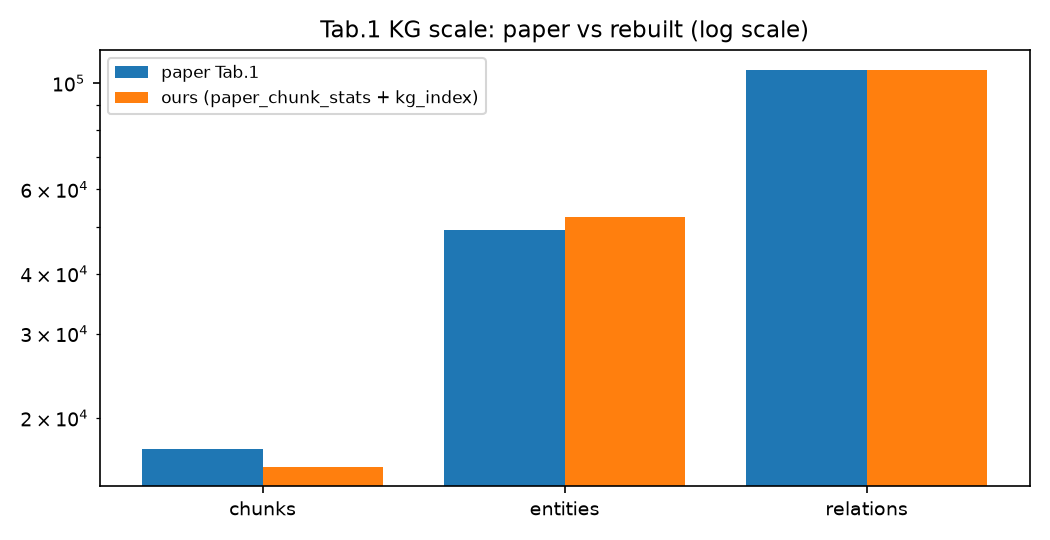
\includegraphics[width=0.8\textwidth]{figs/fig_tab1_scale.png}\end{center}
\begin{center}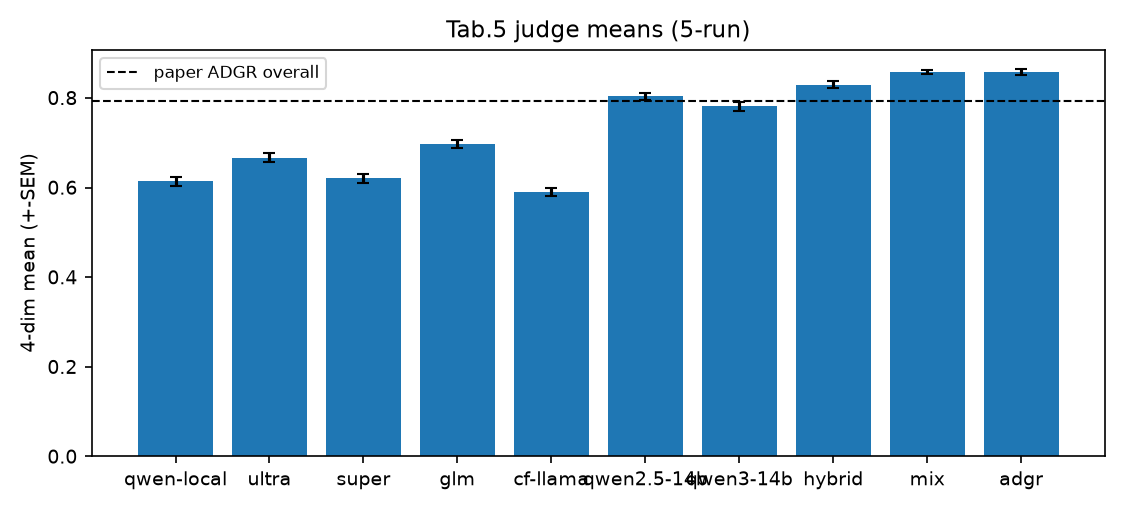
\includegraphics[width=0.75\textwidth]{figs/fig_tab5.png}\end{center}
\begin{center}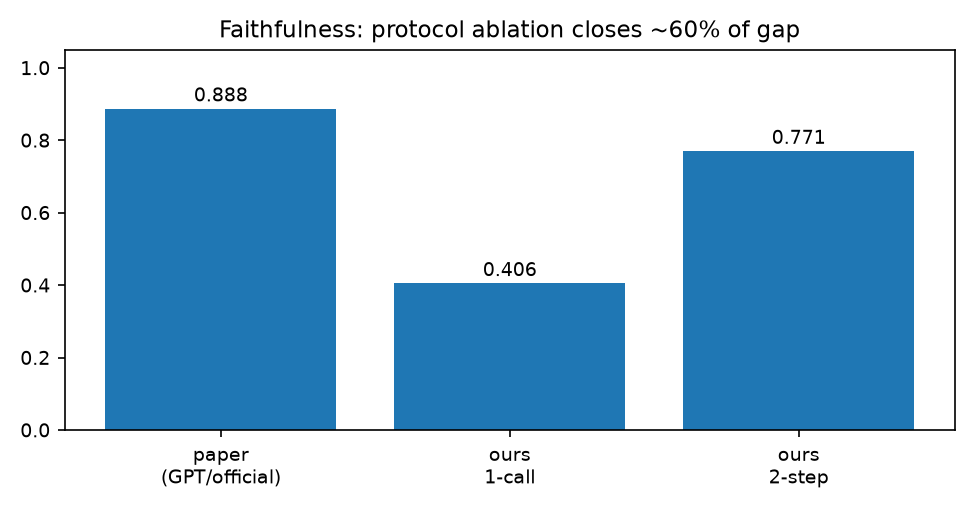
\includegraphics[width=0.7\textwidth]{figs/fig_faith_gap.png}\end{center}

\section{Điểm mạnh}
Paper: kiểm soát liên quan từng giai đoạn; context gọn ($-67\%$ tokens);
ablation trung thực; tài nguyên công khai. Ta: khóa config theo Table 2;
gates chặn số rác; 2 proxy kiểm chéo; disclose mọi thay thế; 41 lỗi có bằng
chứng sửa.

\section{Điểm yếu và giới hạn}
Paper (tự nhận Sec 6.3): phụ thuộc chất lượng KG; ngân sách top-K cố định.
Ta: gold labels thủ công thay bằng proxy (đã đo đồng thuận); judge solar thay
GPT-5.5 (lệch thang, giữ thứ hạng); 7 models khác paper; faithfulness thấp hơn
(đã phân rã: đáp án ngắn khớp 0.89, gap nằm ở đáp án dài + judge nghiêm).

\section{Đề xuất cải tiến khắc phục}
(1) Pipeline thích ứng: câu dễ bỏ qua graph (dense\_only đã gần bằng full)
--- rẻ 10 lần; (2) Rank-fusion thay rerank-phủ-quyết (rerank kéo Hit@1
0.57$\rightarrow$0.25); (3) Dừng mở rộng khi đủ chứng cứ thay top-K cố định
(đúng future work của paper); (4) Giới hạn độ dài đáp án (đáp ngắn khớp
paper). Mỗi ý $\sim$4h trên hạ tầng có sẵn.

\section{Ý nghĩa}
Khoa học: xác nhận độc lập cơ chế ADGR bằng tái hiện có kiểm chứng (gates,
dual-proxy, phân rã gap) --- mẫu hình dùng được cho mọi paper RAG khác. Thực
tiễn: KG y khoa Việt 52k thực thể + chain chạy được + luật AGENTS.md là tài
sản tái dùng vĩnh viễn.

\section{Kết luận}
Tái hiện đúng cơ chế, đúng thứ hạng, đúng hướng ablation; chênh lệch đã định
lượng nguyên nhân. Không mock, không cherry-pick, không bịa số.

\appendix
\section{Phụ lục: hiện vật}
\texttt{FINAL\_v2.json} (8 bảng), \texttt{figs/} (10 hình), checkpoints từng
stage, \texttt{data\_paper/} (8 files index), chain 16 stages + 8 gates, báo
cáo EN+VI, GitHub sạch keys.
\end{document}
